\documentclass[12pt]{article}
\usepackage[utf8]{inputenc}
\usepackage{listings}
\usepackage{amsmath, amssymb}
\usepackage{braket}
\usepackage[margin=1.3in]{geometry}
\usepackage{subfigure}
\usepackage{xcolor}
\usepackage{graphicx}
\usepackage{float}

\title{IBM Quantum Experience Review}
\author{Boettner, Gopalan, Neumann}
\date{May 2020}

\linespread{1.25}

\definecolor{codegreen}{rgb}{0,0.6,0}
\definecolor{codegray}{rgb}{0.5,0.5,0.5}
\definecolor{codepurple}{rgb}{0.58,0,0.82}

\lstdefinestyle{qasm}{
    commentstyle=\color{codegreen},
    keywordstyle=\color{magenta},
    numberstyle=\tiny\color{codegray},
    stringstyle=\color{codepurple},
    basicstyle=\ttfamily\footnotesize,
    breakatwhitespace=false,         
    breaklines=true,                 
    captionpos=b,                    
    keepspaces=true,                 
    numbers=left,                    
    numbersep=5pt,                  
    tabsize=2
}

\lstset{style=qasm}
\newcommand{\url}{\footnote{https://quantum-computing.ibm.com/docs/circ-comp/q-gate}} % too long for body
\newcommand{\qasm}{\footnote{https://github.com/Qiskit/openqasm}}
\newcommand{\ibm}{\footnote{https://thequantumdaily.com/2020/01/30/getting-real-time-information-on-ibm-quantum-devices/}}
\begin{document}

\maketitle
%moved image above chapter and started chapter 1 on a fresh page, it seemed awkward to just have a picture in the beginning of a chapter
\begin{figure}[h!]
        \centering
        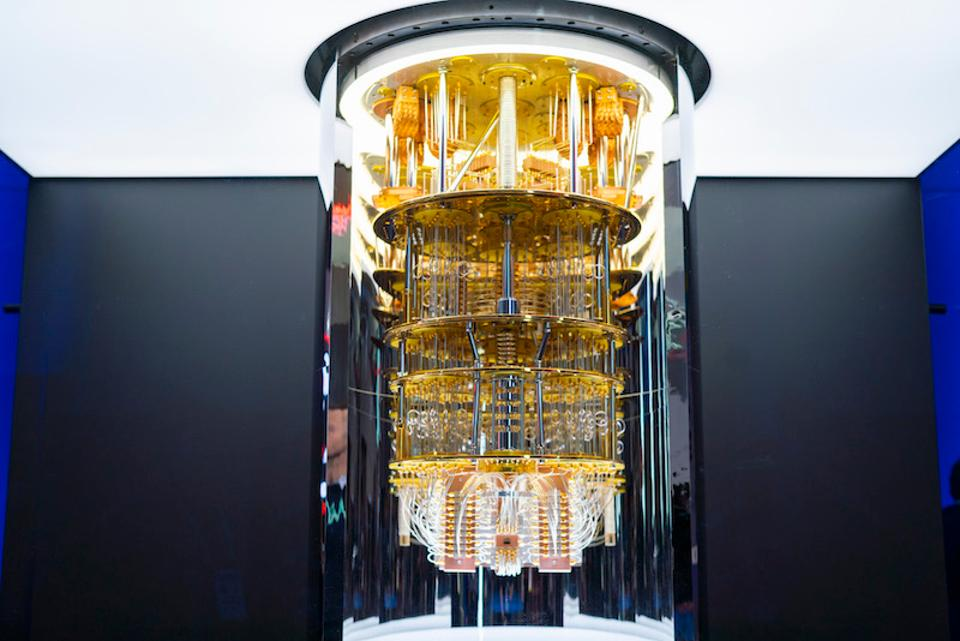
\includegraphics[width=\linewidth]{Circuits/ibm-q.jpg}
        \caption{The IBM Q System One Quantum Computer}
    \end{figure}
    \newpage
\section{The IBM Q System One}
    
    
    %fixed typos and small rewrite of last sentence
    \noindent
    All computing systems rely on a fundamental ability to store and manipulate information. Classical computers manipulate individual bits, which store information as binary 0 and 1 states. Quantum computers instead leverage quantum mechanical phenomena to manipulate information. To do this, they rely on quantum bits, or qubits, which are unit vectors in $\mathbb{C}^2$. Storing and manipulating data in the form of qubits leads to more information. This opens up the possibilities for faster and more efficient algorithms that allow quantum computers to tackle problems that would be harder or practically impossible to solve on a classical computer.
    \\
    \smallskip
    \\
    %maybe describe briefly what shor's algorithm does?
    % shor's is poly time factorization I think? 
    The history of quantum computing research goes all the way back to 1927 and each result marked a new piece of the puzzle. In October 2017, a significant mathematical result was published in the paper “Quantum Advantage with Shallow Circuits” (Bravyi et al. 2018), which guided the development of algorithms for quantum computing. The significance of this algorithm was that unlike Shor’s algorithm, it proved that a quantum computer can solve certain problems with near certainty in a fixed number of steps, no matter the increased input. A classical computer, on the other hand, would require an increased number of steps as the input increases for the same problems. This made the Quantum Advantage algorithm a solid and necessary brick in the foundation of quantum computing.
    \\
    \smallskip
    \\
    %rewrote last sentence
    Building on this foundation, in 2019 IBM Quantum designed and built the world’s first integrated quantum computing system for commercial and educational use: IBM Q System One\ibm\. A large goal of this project was to further quantum computing by providing a reliable resource for quantum research. IBM Q System One provides a superconducting quantum computer that operates outside of research labs allowing the general public to access it for free. In this paper, we describe using the IBM software, recreate circuits to experiment with the Grover’s Search algorithm and the Deutsch-Josza algorithm, and describe our results.

\section{Coding in IBM Q}
    \textbf{IBM Q} was designed to make computing the outcome of Quantum circuits as simple as possible. The built in Circuit Composer allows users to intuitively click and drag universal quantum gates onto a set of qubits. The user can then view the \textbf{QASM} language\qasm \ encoding of their circuit and manipulate it further if they wish. Finally, IBM's cloud based compute model allows the user to run their encoding on one of IBM's servers where it will join a queue before the results of the quantum circuit are sent back to the user. This whole process is highly documented and user friendly. 
    %small rewrites
    This section will outline how to use the Circuit Composer in greater detail as well as provide some simple examples of the interface.
    
    \subsection{Circuit Composer}
        %small rewrites
        The IBM Q Circuit Composer presents the circuit visual as well as the \textbf{QASM} circuit encoding side by side. By allowing user interaction with either, this platform helps the user quickly learn how to tweak their circuit exactly as they want it. This visual interface provides icons for each gate along with a glossary entry for each icon that explains what the gate does. Despite providing the option to write code, the Circuit Composer in no way forces the user to have past programming experience. The QASM representation simply allows more precise control over the circuit creation process.
        
        \begin{figure}[ht]
            \centering
            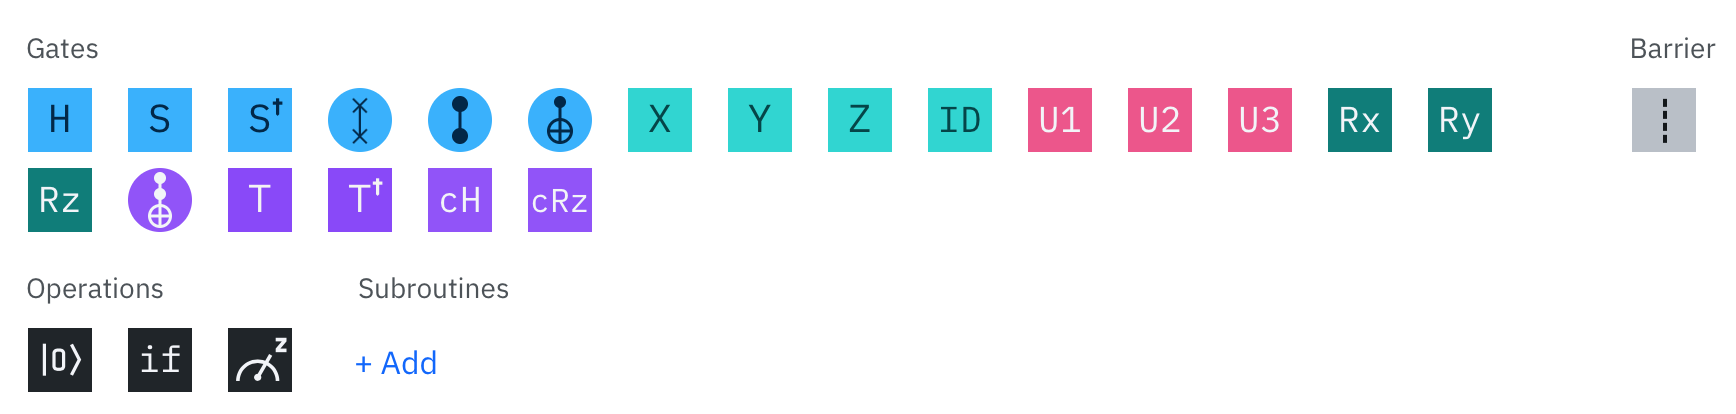
\includegraphics[width=\linewidth]{Circuits/gates.png}
            \caption{Gates in the Circuit Composer}
        \end{figure}
        
    \subsection{Encoding}
        %small rewrites
        Circuit encoding in IBM Q is simple. The software uses the QASM language developed by IBM in 2017 and uses arrays to represent qubit input states. The QASM provides a set of quantum gates that are represented with letters and take qubits as inputs. The order in which these gates appear in the code correlates to the order that they appear on the circuit. This encoding can then be interpreted by the IBM servers in order to compute the results of the circuit.
        \\
         \smallskip
        \\
        Encoding each circuit into a small file is a crucial element of IBM Q software for a number of reasons. Most importantly, the simplified and optimized encoding helps combat the severe limitations of our current quantum computing capabilities. The optimization occurs when IBM transpiles\footnote{The transpiler introduces the concept of a pass manager to allow users to explore optimization and find better quantum circuits for their given algorithm (Qiskit 20).} the circuit encoding. In this process, the number of quantum gates is reduced as much as possible while maintaining the circuit's properties. Additionally, the small file size minimizes data transfer between users and IBM servers which allows faster and more convenient access for everyone.

    \subsection{Getting Results}
        %small rewrites
        As previously mentioned, IBM Q is fully cloud based. This system utilizes multiple global servers to process user circuits. When a user submits their circuit to be run a specified number of times, it joins a server queue. These servers utilize classical computers to decode the quantum circuit and send the corresponding qubits to a real quantum computer. The quantum computer then runs the circuit as many times as specified and returns the results back to the user. The results use a histogram to display each returned state along with probability with which that state appeared. These results also include the time it took for the circuit to transpile, validate, queue, and run.
        
        
\section{Theory}
    \subsection{Deutsch-Jozsa algorithm}
    %first sentence here is kinda funky, not sure how to fix because I'm not sure what it's saying
    %small rerwrites
    The Deutsch-Jozsa algorithm was one of the first quantum algorithms to show a separation between the quantum and classical difficulty of a problem. Formally, it is defined as follows: Consider a function $f(x)$ that takes as input $n$-bit strings $x$ and returns 0 or 1. We are promised that $f(x)$ is either a \emph{constant} function that takes the same value $c \in {0,1}$ on all inputs $x$, or a \emph{balanced} function that takes each value 0 and 1 on exactly half of the inputs. \textbf{The goal is to decide whether $f$ is constant or balanced by making as few function evaluations as possible}. 
    \\
    \smallskip
    \\
    %rewrites
    Our class performed a simple implementation of the Deutsch-Jozsa algorithm in which we used the `phase kickback trick' for an oracle to guess the sum of two bits using only a single query. Classically this would take 2 queries. %i don't understand the next sentence
    In our tests with the IBM software, we implement a more `quantum-like' experimental setup that is described \textbf{here}\footnote{see https://quantum-computing.ibm.com/docs/guide/q-algos/deutsch-jozsa-algorithm}. In this setup, consider a typical interference experiment where a particle that behaves like a wave, such as a photon, can travel from the source to an array of detectors by following two or more paths simultaneously. The probability of observing the particle will be concentrated at those detectors where most of the incoming waves arrive with the same phase. 
    We can set up the $2^n$ possible paths and $2^n$ detectors with $n$-bit strings $x$ and $y$ where $x$ denotes a path and $y$ denotes a detector. Though this experiment is not practical since it would require an impossibly large optical table, we can simulate this experiment on a quantum computer with just $n$ qubits and access to the oracle circuit $U_f$. Classically, this method requires $2^{n-1}+1$ function evaluations in the worst case, but using the Deutsch-Jozsa algorithm the question can be answered with just one function evaluation.
    \\
    \smallskip
    \\
    Suppose that the phase accumulated along a path $x$ to a detector $y$ equals $C(-1)^{f(x)+x.y}$ where $x.y = \sum_{i=1}^{n} x_{i}y_{i}$ is the binary inner product and $C$ is a normalizing coefficient. The probability to observe the particle at a detector $y$ can be computed by summing up amplitudes of all paths $x$ arriving at $y$ and taking the absolute value squared, i.e.,:
    \begin{equation}
        Pr(y) = \mid C\sum_{x}(-1)^{f(x)+x.y} \mid^{2}
    \end{equation}
    
    \noindent
    %small rewrites
    The normalization condition, $\sum_{y}Pr(y) = 1$, gives us $C = 2^{-n}$. Now, we can compute the probability  of observing the particle at the detector $y = 0^n$ (the all zeros string). We have $Pr(y=0^{n}) = \mid2^{-n}\sum_{x}(-1)^{f(x)}\mid^2$. If $f(x) = c$ is a constant function, we get $Pr(y=0^{n}) = \mid(-1)^c\mid^2 = 1$. However, if $f(x)$ is a balanced function, we get $Pr(y=0^{n}) = 0$, since all terms in the sum cancel each other out. We can therefore determine whether $f$ is constant or balanced with certainty by running the experiment just once. The Deutch-Josza algorithm is as follows:
    
    \begin{enumerate}
        \item Initialize $n$ qubits in the all-zeros state $\ket{0,0,\cdots,0}.$
        \item Apply the Hadamard gate $\mbox{\em{H}}$ to each qubit.
        \item Apply the oracle $U_{f}$.
        \item Repeat Step 2.
        \item  Measure each qubit. Let $y = (y_1, \cdots, y_n)$ be the list of measurement outcomes. We find that $f$ is a constant function if $y$ is the all-zeros string.
    \end{enumerate}
    
    \noindent
    %small rewrites
   The applications of Hadamards in Step 4 maps a basis state  to a superposition $2^{-n/2}\sum_{y}(-1)^{x.y}\ket{y}$. Thus the state reached after Step 4 is $\ket{\Psi} = \sum_{y}\Psi(y)\ket{y}$, where $\Psi (y) = 2^{-n}\sum_{x}(-1)^{f(x)+x.y}$. This is exactly what we need for the interference experiment described above. The final measurement at Step 5 represents detecting the particle. The probability to measure in Step 5 is 1 if $f$ is a constant function and 0 if $f$ is a balanced function. Thus the Deutsch-Jozsa problem is solved with certainty by making just one function evaluation.
    
    
    
    \subsection{Grover Search algorithm}
    % I rewrote the intro sentence 
    %rewrote some more
    One major benefit of Quantum computers is the ability to search databases much faster than classical computers. The Grover's search algorithm is a great example of how quantum computers obtain this advantage. When applied in an unstructured search, Grover's Search algorithm can speed up the problem quadratically. The experiments described in this paper are modeled on the resource notes provided \textbf{here}\footnote{see https://quantum-computing.ibm.com/docs/guide/q-algos/grover-s-algorithm}. 
    \\
    \smallskip
    \\
    %all of the rewrites
    In essence, an unstructured search is the task of finding a desired item within an unordered list of $N$ items. In classical computing, this search takes $N$ steps in the worst case scenario and $N/2$ steps on average. A quantum computer using Grover's Search algorithm can reduced this search to $\sqrt{N}$ steps. An additional benefit of Grover's search algorithm is that it does not require the list to have a specific internal structure. This makes the algorithm a general solution for a wide variety of database search problems.
    \\
    \smallskip
    \\
    %there was no mention as to what x and w represent here so I added a small intro and rewrote rest accordingly
    Consider an unstructured list of $N$ items. Each item is denoted $x$ except the item we are searching for which will be denoted $w$. The tactic used to search this unstructured list exploits Grover’s amplitude amplification trick by repeatedly applying an oracle $U_f$ and rotating about a superposition state. This oracle encodes all items within the list as a function $f$ which returns $f(x) = 0$ for all $x \neq w$ and $f(x) = 1$ for $x$ = $w$. This function is encoded as a unitary matrix which allows a quantum computer to interpret each item as a superposition to the function. Here, for the basis states $\ket{x}$, the $U_f$ unitary matrix is given as $U_f \ket{x} = (-1)^{f(x)} \ket{x}$.
    \\
    \smallskip
    \\
    Since $w$ could be anywhere within the list, the general strategy is to try the uniform superposition state as input for the oracle: $$\ket{s} = \frac{1}{\sqrt{N}}\sum^{N-1}_{x=0}\ket{x}$$
    \noindent
    When we measure this state, we measure all states with equal probability (1/$N$). This is where amplitude amplification comes in. The algorithm utilizes geometrical interpretations of two reflections, which generate a rotation in a two-dimensional plane. The only two special states we need to consider are the desired item $\ket{w}$,  and the uniform superposition $\ket{s}$. Though these two vectors span a two-dimensional plane in the vector space $\mathbb{C}^2$, they are not quite perpendicular. Thus we introduce an additional state $\ket{s^\prime}$  that represents the span of these two vectors, which is perpendicular to $\ket{w}$ and is obtained from $\ket{s}$ by removing $\ket{w}$ and re-scaling. The Grover’s Search algorithm is as follows:
    
    \smallskip
    
    \begin{enumerate}
        \item  Start with the uniform superposition state $\ket{s}$. $\ket{\psi_0} = \ket{s}$
        \item Apply the oracle $U_f$ to the state $U_f \ket{\psi_t} = \ket{\psi_t'}$
        \item Apply another rotation $U_s$ about $\ket{s}$ using $U_s = 2\ket{s}\bra{s}-1$, giving us $\ket{\psi_{t+1}} = U_{s}U_{f}\ket{\psi_t}$
        \item Repeat step 2.
    \end{enumerate}
    \noindent
    %this first sentence doesn't really make sense given it's context
    %some rewrites
    The two reflections result in a rotation. The transformation $U_{s}U_f$ rotates the initial state $\ket{s}$ closer towards the desired item $\ket{w}$. Since the average amplitude has been lowered by the first reflection, this transformation boosts the negative amplitude of $\ket{w}$ to roughly three times its original value, while it decreases the other amplitudes. Step 2 is then repeated several times which allows the algorithm to get closer and closer to the desired item $\ket{w}$. After $t$ steps we have $\ket{\psi_t} = U_{s}U_{f} \ket{\psi_0}$. After roughly $\sqrt{N}$ rotations, the algorithm will zero in on $w$, as we can see that the amplitude of $\ket{w}$ grows linearly with the number of applications $\approx tN^{-1/2}$.
        
\section{Expressing Circuits in IBM Q}
    %some rewrites
     For both Deutsch-Jozsa and Grover's Search algorithms, IBM had included numerous examples of their equivalent circuits. We decided to test these examples to see if they held up to their theoretical results. Using the given examples allowed us to test IBM's implementations and makes sure there were no errors in our own encoding. We verified that these encodings matched the algorithms from our notes and then ran them multiple times through the IBM servers. The subsections bellow detail our results.
    
    \subsection{Deutsch-Jozsa algorithm}
        For this example we tested a constant and balanced function with the Deutsch-Jozsa algorithm. IBM's example for a balanced function over three qubits uses Hadamard gates, a C-not and a controlled Z-gate. This function should never return the all zero state. In contrast, the constant function example simply Hadamards each qubit twice with no function in the middle (this is clearly a constant function as it is the Deutsch-Jozsa of the trivially constant function). When the first example circuit is run through the IBM Q software, it returned even results for each state but the all zero qubit state. This suggests that the function is balanced since the Deutsch-Jozsa algorithm never returns the string of all zeros. In contrast, for the trivial constant function the result was always the state of all zero qubits. This clearly shows that the software correctly evaluated both example circuits. We ran these simulations multiple times without error or false positives. This demonstrates that the quantum computer can reliably evaluates these circuits.
        \begin{figure}[ht]
            \centering
            \begin{minipage}{0.35\linewidth}
                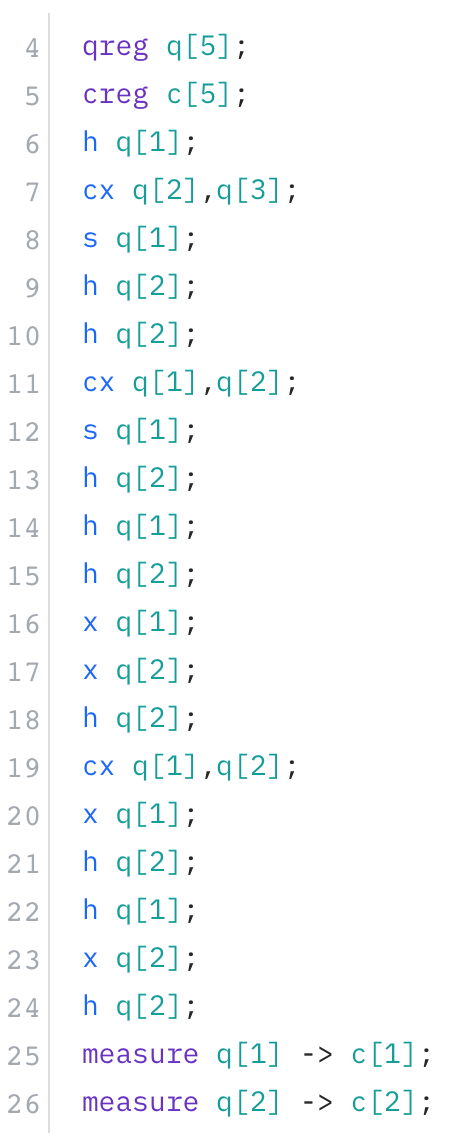
\includegraphics[width=\linewidth]{Circuits/Deutsch-Jozsa-code.png}
            \end{minipage}%
            \begin{minipage}{0.65\linewidth}
                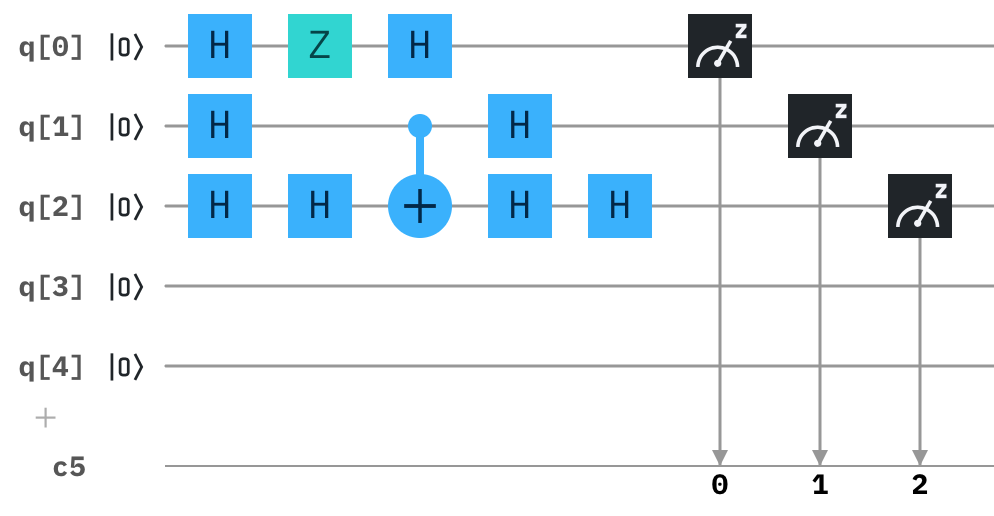
\includegraphics[width=\linewidth]{Circuits/Deutsch-Jozsa.png}
            \end{minipage}
            \caption{Deutsch-Jozsa on Balanced Function}
        \end{figure}
        \begin{figure}[ht]
            \centering
            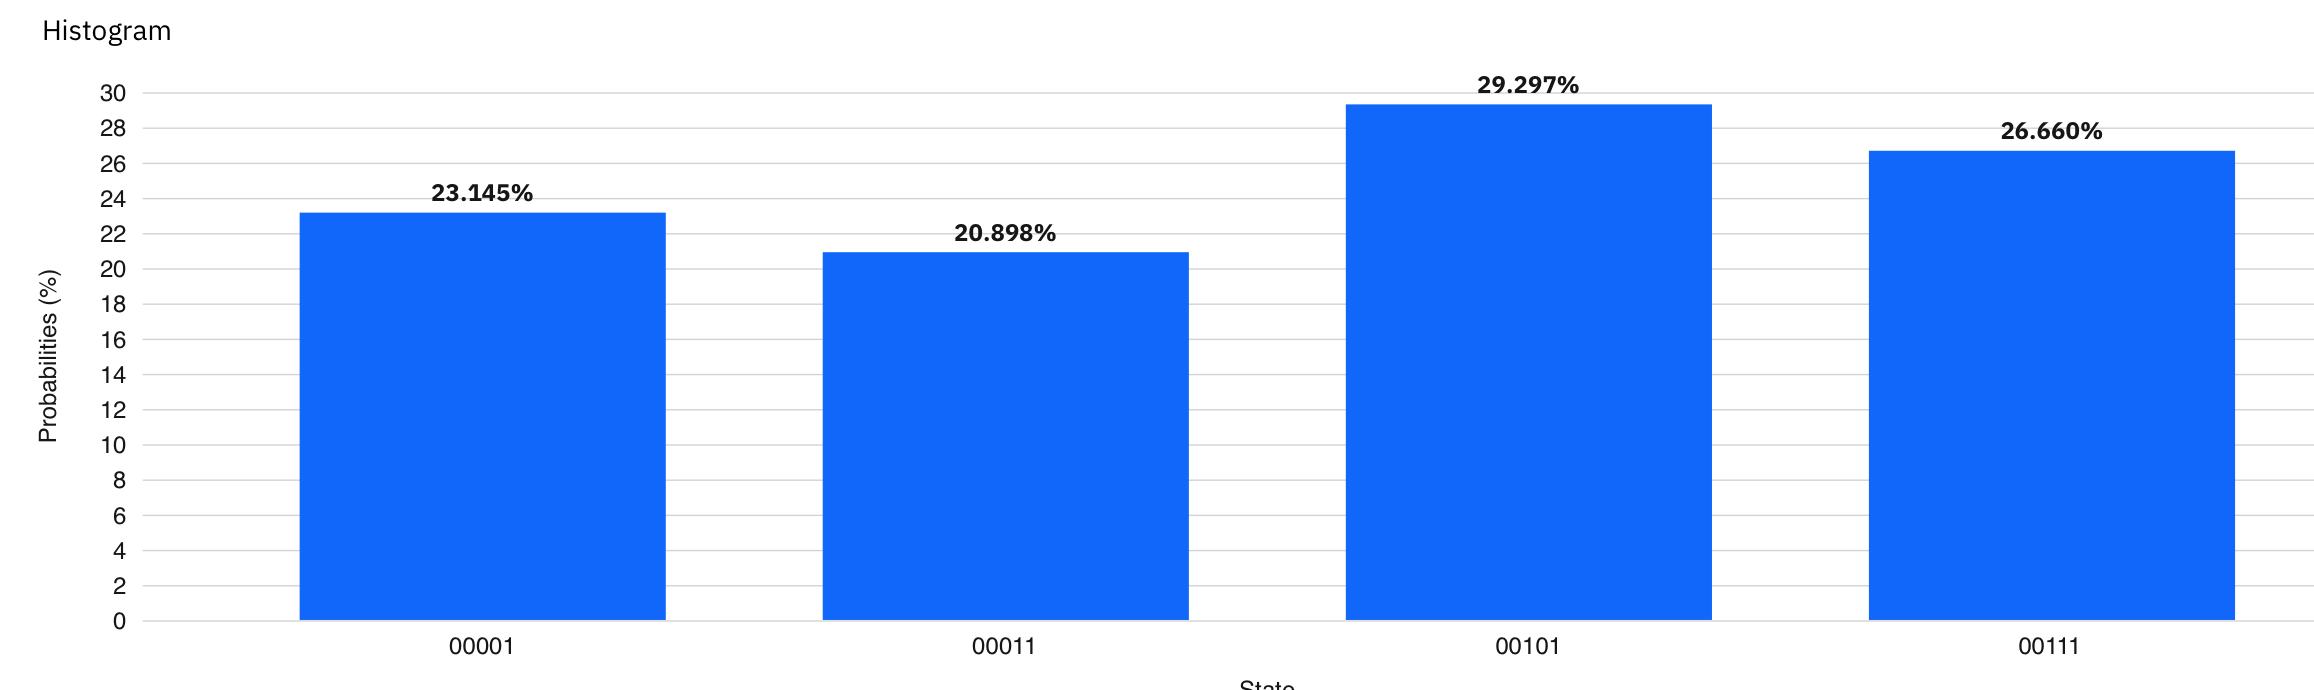
\includegraphics[width=\linewidth]{Circuits/Deutsch-Jozsa-result.png}
            \caption{Result for Balanced Function}
        \end{figure}
        \begin{figure}
            \centering
            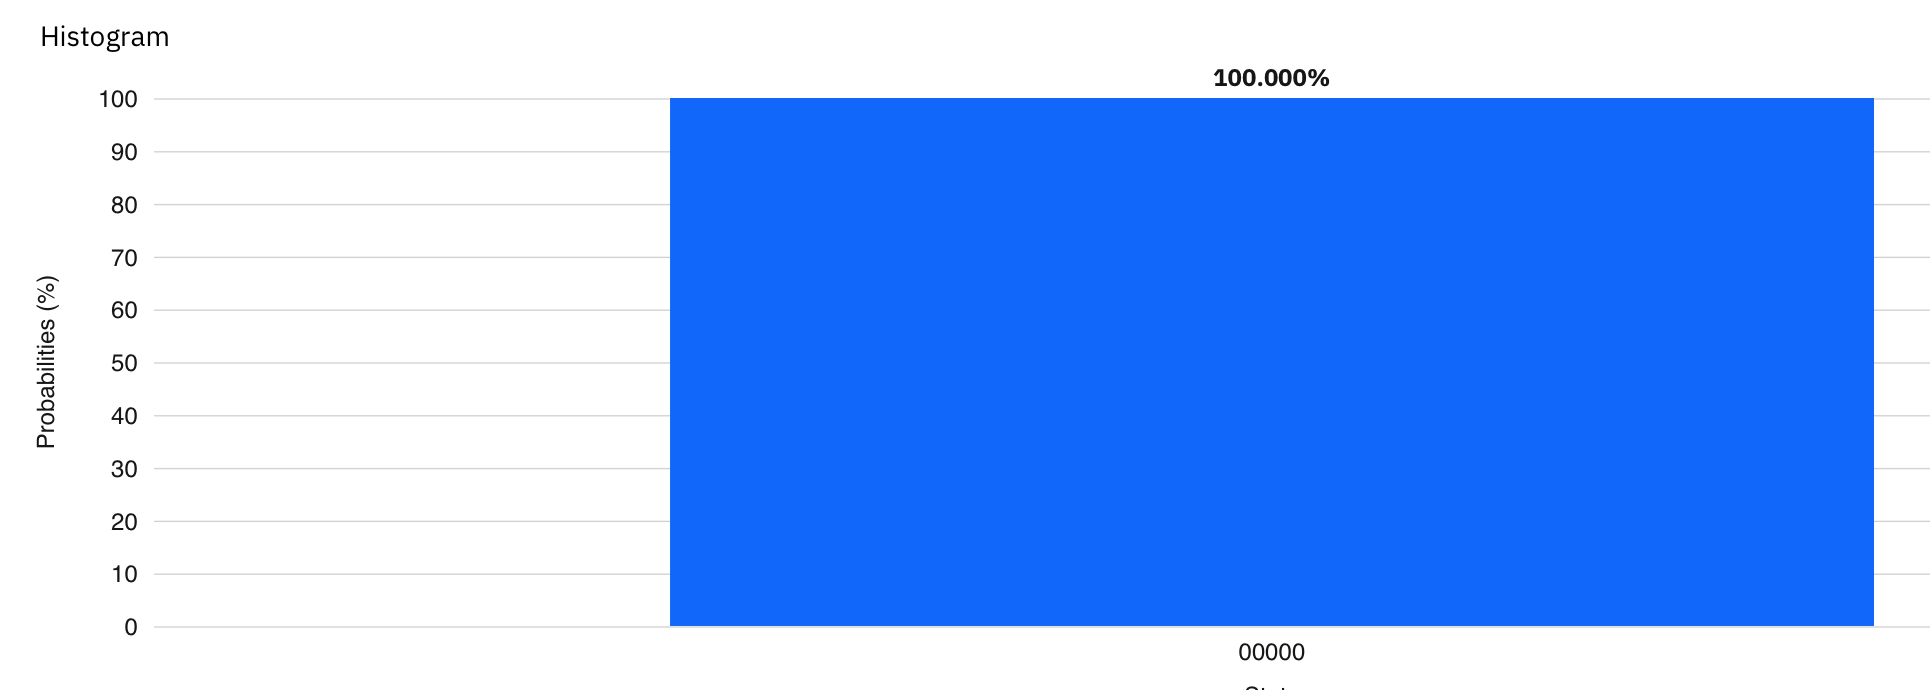
\includegraphics[width=0.6\linewidth]{Circuits/Deutsch-Jozsa-result2.png}
            \caption{Result for Constant Function}
        \end{figure}
    \subsection{Grover Search algorithm}
        %small fixes/trimming
        The Grover search algorithm finds a given element inside of a list or database. As mentioned in the theory section, the number of necessary oracles for an n-qubit state is $\sqrt{n}$. For the example IBM provided, there are two qubits and four necessary oracle circuits. Each of these circuits corresponds to a given output state and if the quantum computer works properly, they would each only return one result with high probability. In this case IBM Q interpreted the four oracle circuits correctly and each only returned the expected state. This suggests that the software properly evaluated each circuit and that their example of the Grover search algorithm matched the one we studied in class.
        \begin{figure}[h!t]
            \centering
            \begin{minipage}{0.35\linewidth}
                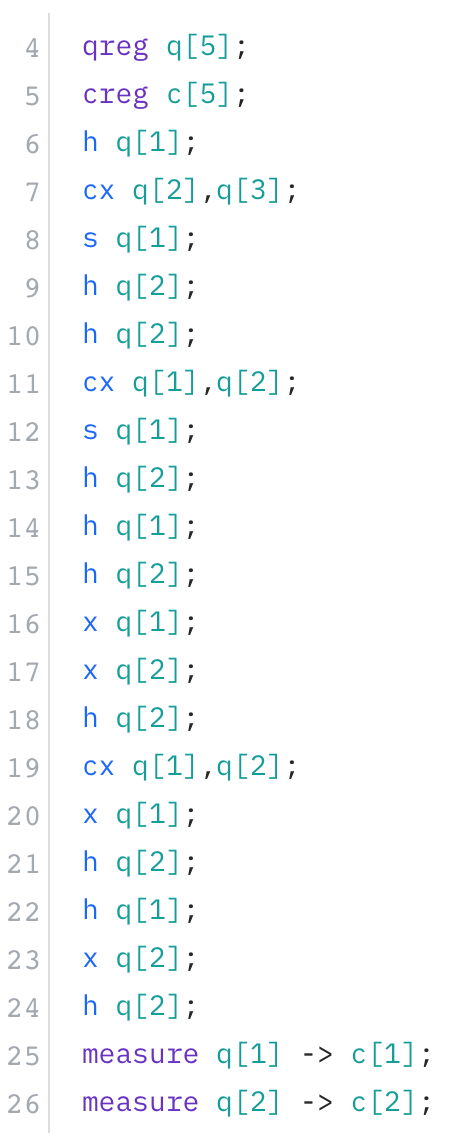
\includegraphics[width=\linewidth]{Circuits/grover-code.png}
            \end{minipage}%
            \begin{minipage}{0.65\linewidth}
                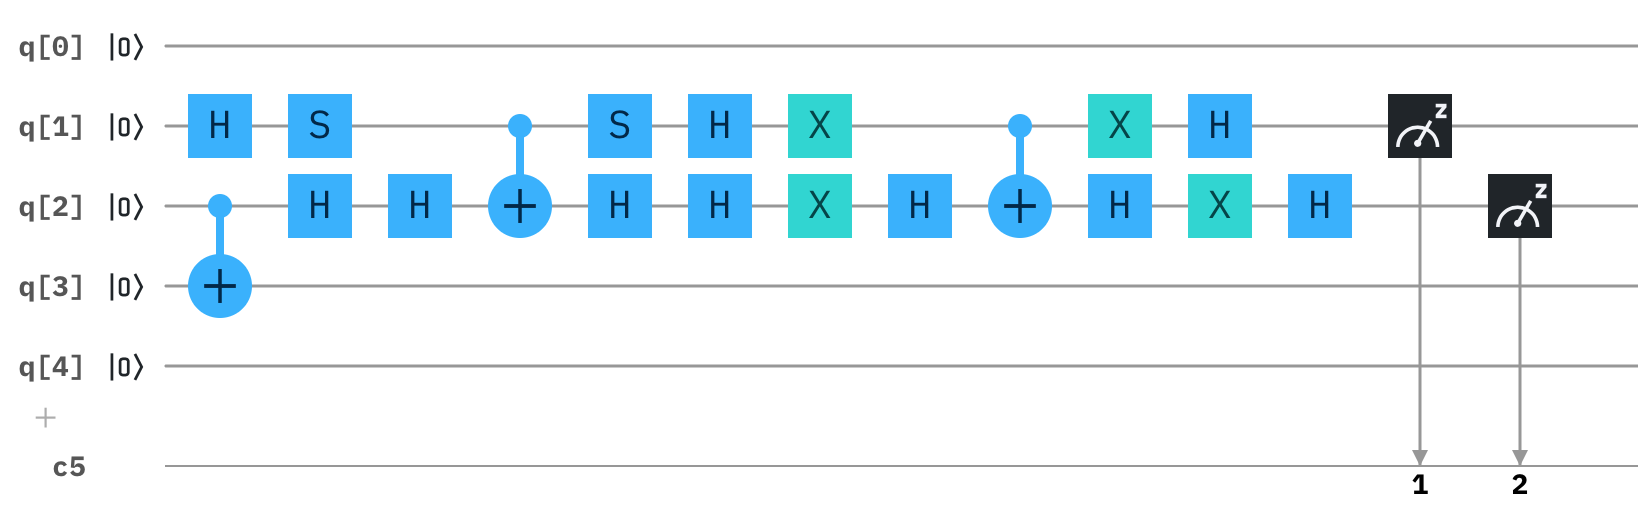
\includegraphics[width=\linewidth]{Circuits/grover.png}
            \end{minipage}
            \caption{Grover Search algorithm (a)}
        \end{figure}
        %just used new page here to put diagram on the right page
        \newpage
    
\section{Conclusion}
    There are still many obstacles to overcome before achieving general purpose quantum computing. In order to distinguish between states and make any sort of calculation, a two level system is required. While bits in classical computing can be easily flipped and distinguished, physical qubits are extremely volatile and will rapidly decay their energy into the environment. The current most promising method of maintaining a two level system with superconducting qubits is to keep them at extremely low temperatures. For example, the IBM Quantum Experience keeps its superconducting qubits at 15 milliKelvin in order to reduce ambient heat and noise from interfering with the system. Despite this, our current technology and understanding only allows qubits to be maintained at an excited state for a small number of microseconds. Thus any quantum computation that takes longer than a small number of microseconds will become meaningless. This severely limits the current potential of quantum computers in tackling practical problems.
    \\
    \smallskip
    \\
    %trimmed off some parts
    Due to this severe limitation, quantum computing does not currently have many general purpose abilities. While the IBM quantum computer is fascinating to experiment with and prove various results, its computational power is quite limited. The IBM Q software was designed to allow academics and engineers to test circuits on an actual quantum computer and further software development with quantum algorithms. While the current IBM quantum computer does not provide practical benefits, it still benefits our understanding of quantum computation for when quantum computers become more accessible. IBM's software is easy to approach and use while still allowing for more complicated research and application. This paper only skims the surface of IBM's potential. Further research and testing will reveal the full capability of IBM's quantum software.
    
    

\newpage

\section{Appendix}
\subsection{Qiskit}
        %small fixes
        Qiskit is a framework developed around QASM to make it possible to work with IBM Q from a console. For the purposes of this project we didn't create any Qiskit files, but it would be very useful for future research. This framework can be installed as a Python library through the pip package manager. When a user inputs their API key for the IBM Q software they can send any QASM circuit to one of the backend servers for processing. The server responds with a dictionary of each possible qubit state and the number of runs that resulted in that state. This interface allows for more nuanced work and allows a user to save configuration and circuit settings between queries. For the average user, Qiskit adds a lot of unnecessary complexity and code to the process of drawing and testing a quantum circuit. For researchers and engineers however, it allows far more flexible configurations and setups for testing quantum circuitry. We would highly recommend the Qiskit framework for work utilizing the IBM Q quantum computing platform.

\end{document}

